\documentclass{article}
\usepackage{tikz}[standalone]
\usetikzlibrary{knots}
\begin{document}
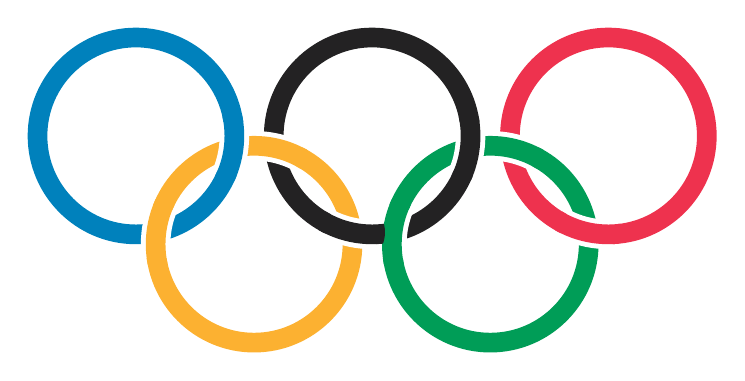
\begin{tikzpicture}
\definecolor{blue1}{RGB}{0,129,188}
\definecolor{yellow1}{RGB}{252,177,49}
\definecolor{black1}{RGB}{35,34,35}
\definecolor{green1}{RGB}{0,157,87}
\definecolor{red1}{RGB}{238,50,78}
\begin{knot}[clip width=1.5pt]
    \strand[line width=0.25cm,red1] (3,0) circle(1.25cm);
    \strand[line width=0.25cm,green1] (1.5,-1.375) circle(1.25cm);
    \strand[line width=0.25cm,black1] (0,0) circle(1.25cm);
    \strand[line width=0.25cm,yellow1] (-1.5,-1.375) circle(1.25cm);
    \strand[line width=0.25cm,blue1] (-3,0) circle(1.25cm);
    \flipcrossings{2,4,6,8}
\end{knot}
\end{tikzpicture}
\end{document}
